<<<<<<< Updated upstream
Decadal Testbed Paper:

Ames Coronagraph Experiment (ACE)
-designed to develope the PIAACMC coronagraph
-using a single MEMS DM
-two sources to simulate a binary star system
-experiments include maintaining raw contrast with LDFC, wavefront and control techniques to dig dark holes on a field with multiple stars

Belikov et al. 2012

High-Contrast High-Resolution Spectroscopy for Segmented Telescopes (HCST).
-Caltech

-testing vortex coronagraphs Ruane et al. 2018b
-BMC DM, possibly two by now
-clear aperature
-linking coronagraphs and spectrographs with single mode fibers
Llop Sayson, et al. 2019)

High contrast imager for complex aperture telescope (HiCAT)
-space telescope science institute
-study the impacts that the shape of the pupil aperture has on high contrast. things light spiders and obscurations. 
-segmented DM, two MEMs Dm
-Aopodized Pupil Lyot Coronagraph

Très Haute Dynamique 2 (THD2)
Paris Observatory
two 32x32 MEMs DMs

360 degree dark hole with clear aperture
-phase mask coronagraphs
-wavefront control techniques

% Goal: want to look for life on other planets
% Problem: High contrast issue. Planets faint. Planets small. Atmospheric         turbulence degrades resolution.
% Solution: ExAO and coronagraphy.
%     Exao works by:
%     coronagraphy works by:

% Goal: want to build giant telescopes because they will actually be able to     image Exo-Earths
% Problem: need to further develop current exao and coronagraph techonology,     to reach and maintain the needed contrasts  
% Solution: Testbeds from institutions around the world dedicated to             coronagraphy and exao research.

% Corongraph testbeds:
%     -vapp
%     -vector
%     -PIAA
%     -lyots
    
% Exao testbeds:
%     -predictive control
%     -speckle nulling
%     -LDFC, EFC
%     -improving current WFS by:
%         -optimizing WFS
%         -investigating better WFS (zernike)
%         -developing multistage WFS control (LOWFS, high order)
        
% Our Solution:
%     -robust testbed for multiple experiments
%     -talk about current experiment to explore and alternative WFS






% \jrmcom{I would make the opening sentence more broad.  It's about all high contrast imaging, which is more than the search for life, even more thane exoplanets.  Then you highlight that searching for life is the ultimate goal requiring the most demanding performance} 

% The search for life and habitable words beyond our solar system is a driving force of modern astronomy and one of the most captivating questions of our time. 
% To study exoplanets astronomers use a technique called high contrast imaging which is a type of direct imaging.  
% -add more on exoplanet science. 


%  High contrast imaging with astrometric calibration allows an astronomer to make precise measurements of the exoplanet’s period and orbit.\cite{seager2010exoplanets} \jrmrmv{In combination with a spectrograph, we can directly measure the atmospheric composition of exoplanets to look for signatures of organic molecules and liquid water}\jrmcom{move before astrom and make general}.\cite{seager2015search}

% % DONT INCLUDE. 
% \begin{figure}
% \begin{center}
% 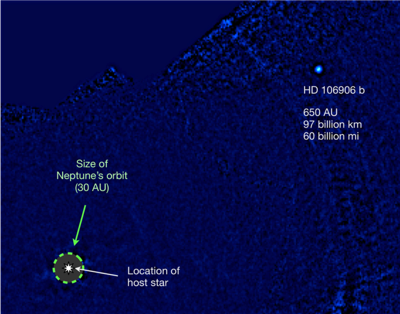
\includegraphics[width=0.6\textwidth]{exoplanet.png}
% \caption{Image of exoplanet HD 106906 b taken with the Magellan Adaptive Optics (MagAO) instrument. \cite{bailey2013hd}}
% \label{fig:exoplanet}
% \end{center}
% \end{figure}


% Our ability to study exoplanets is limited by the high contrast problem; exoplanets are much fainter than stars and cannot be detected without starlight suppression. In direct imaging we are detecting the exoplanet’s thermal emission, and the starlight reflected off \jrmrmv{of} the exoplanet’s atmosphere\cite{seager2010exoplanets} which is dwarfed by that of the host star. For example, the contrast between the Sun and the Earth is on order $10^{-10}$ in the visible spectrum \jrmcom{also give what it is at 10 um since you intro-ed thermal}. \jrmcom{What are you trying to say here?  It's true by definition in teh previous sentence -- so what point?} This extreme contrast ratio is the same for Earth-sized exoplanets in the habitable zone, and improves to $10^{-8}$ contrast for exoplanets around M-dwarf stars\cite{males2014direct}.  Ground based observatories face additional challenges from aberrations caused by atmospheric turbulence that degrades the resolution of the image making the detection of the exoplanet more challenging. 
=======
3PWFS Pupil size:
Q3: 29.5
Q2: 29.35
Q1: 29.4

4PWFS Pupil Size:
Q1: 30.5
Q2: 30.7
Q3: 30.7
Q4: 30.5

3PWFSSM: 498 modes
>>>>>>> Stashed changes
